\chapter{Cahier des charges - MVP 1}

\section{Introduction}
Le premier MVP (Minimum Viable Product) du projet \textbf{OrganisX} vise à développer une application web simple de gestion de tâches personnelles (type Todo list). 
Ce MVP permettra de valider les choix techniques, d’expérimenter l’architecture hexagonale mise en place et de tester l’expérience utilisateur de base avant d’ajouter des fonctionnalités avancées (notifications, paiements, gestion d’équipes, etc.).

\section{Objectifs du MVP 1}
\begin{itemize}
	\item Fournir un système d’authentification basique (inscription et connexion).
	\item Permettre à un utilisateur connecté de créer, consulter, modifier et supprimer ses propres tâches.
	\item Assurer une séparation claire entre le frontend (Angular) et le backend (ASP.NET Core en architecture hexagonale).
	\item Préparer le terrain pour l’évolutivité (microservices futurs, ajout d’équipes, etc.).
\end{itemize}

\section{Périmètre fonctionnel}
Le MVP 1 inclut uniquement les fonctionnalités essentielles listées ci-dessous.

\subsection{Périmètre, acteurs et scénarios}
\subsubsection{Acteurs principaux}
\begin{tabular}{|l|p{10cm}|}
	\hline
	\textbf{Acteur} & \textbf{Description} \\ \hline
	Utilisateur non authentifié & Peut s'inscrire ou se connecter \\ \hline
	Utilisateur authentifié & Gère ses tâches personnelles \\ \hline
	Système d'authentification & Émet et valide les jetons, applique les politiques de sécurité \\ \hline
\end{tabular}

\subsection{Cas d’utilisation principaux}
\begin{itemize}
	\item \textbf{UC1 - S’inscrire :} L’utilisateur crée un compte en fournissant un email et un mot de passe.
	\item \textbf{UC2 - Se connecter :} L’utilisateur accède à l’application via email et mot de passe. 
	\item \textbf{UC3 - Créer une tâche :} L’utilisateur ajoute une nouvelle tâche avec un titre, une description (optionnelle) et une date d’échéance.
	\item \textbf{UC4 - Lister mes tâches :} L’utilisateur visualise toutes ses tâches, triées par date de création ou échéance.
	\item \textbf{UC5 - Modifier une tâche :} L’utilisateur met à jour le titre, la description, l’échéance ou l’état d’une tâche (À faire, En cours, Terminé).
	\item \textbf{UC6 - Supprimer une tâche :} L’utilisateur supprime une tâche définitivement.
\end{itemize}

\subsection{Diagramme d’utilisation (optionnel)}
\begin{figure}[H]
	\centering
	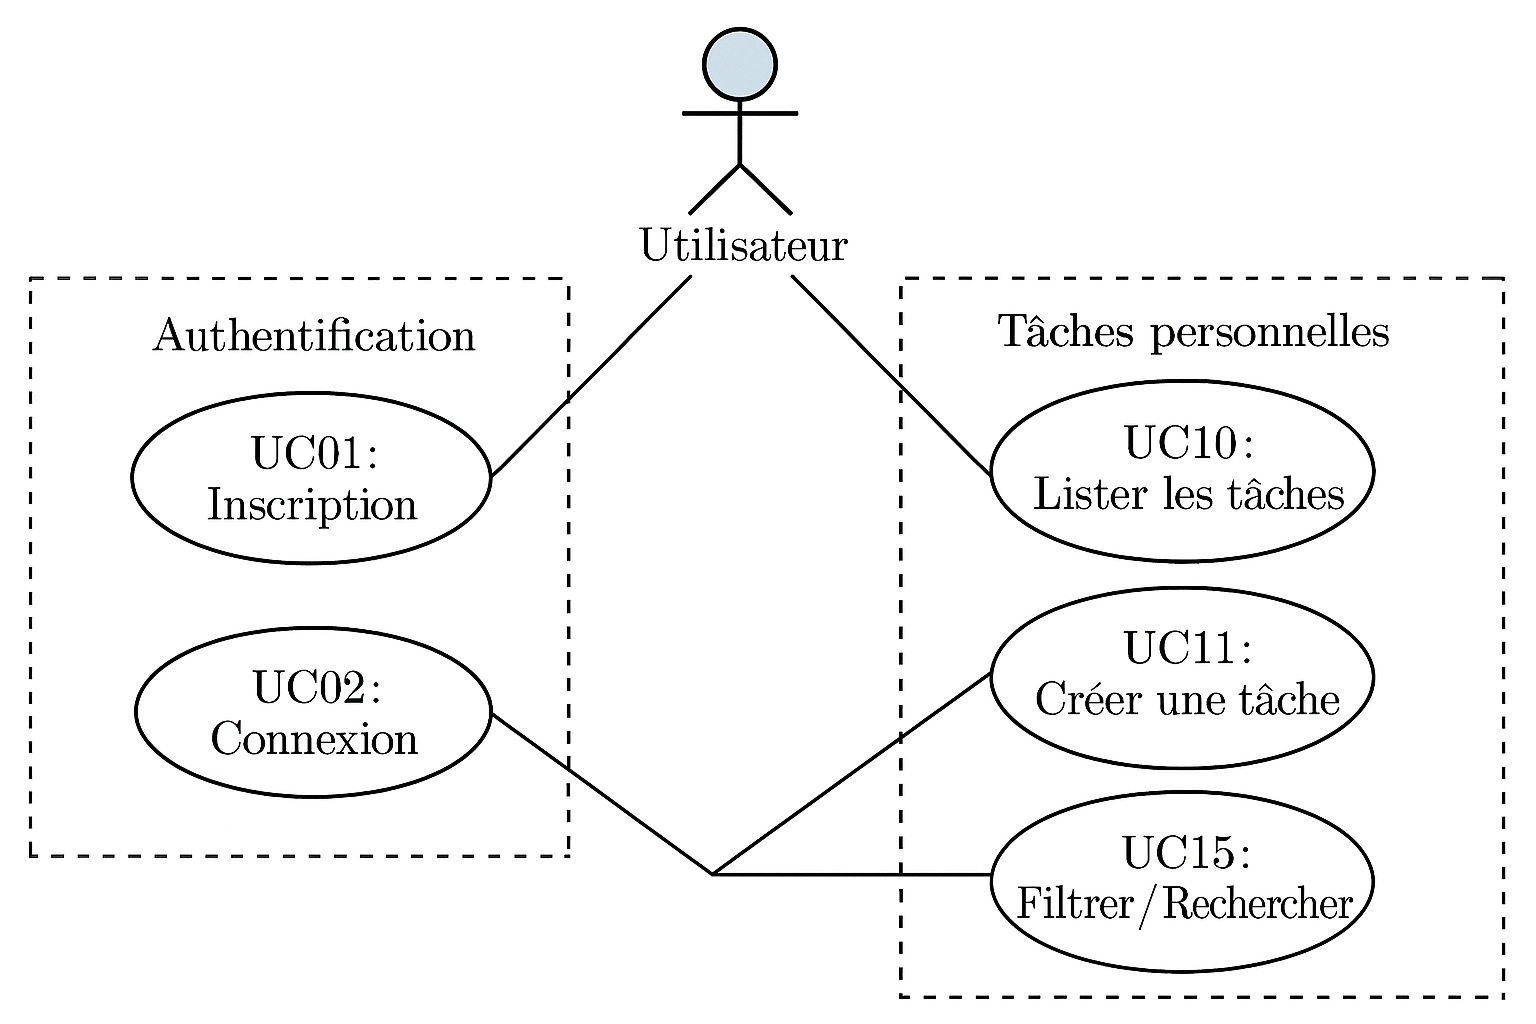
\includegraphics[width=0.8\textwidth]{images/diagram_use_cases.png}
	\caption{Diagramme des cas d’utilisation du MVP 1}
\end{figure}

\subsection{Paramètres et données}
\begin{itemize}
	\item \textbf{Personnalisation de l’affichage} : Choix du thème, langue et préférences d’interface.
	\item \textbf{Export des données} : Export des tâches au format CSV ou JSON.
\end{itemize}

\section{Exigences techniques}
\subsection{Backend}
\begin{itemize}
	\item Langage : C\# avec .NET 9.
	\item Architecture : Hexagonale (Domain, Application, Infrastructure, API).
	\item Base de données : PostgreSQL.
	\item Sécurité : Authentification JWT.
	\item Tests unitaires : xUnit.
\end{itemize}

\subsubsection{Modèle de données simplifié}
\begin{tabular}{|l|p{5cm}|p{6cm}|}
	\hline
	\textbf{Entité} & \textbf{Attributs} & \textbf{Contraintes} \\ \hline
	Utilisateur & id, email, passwordHash, displayName, locale, timeZone, createdAt & Email unique, mot de passe hashé \\ \hline
	Tâche & id, userId, title, description, status, priority, dueDate, tags[], createdAt, updatedAt & FK userId, taille max description 2000 caractères \\ \hline
\end{tabular}

\subsubsection{API principales}
\begin{description}
	\item[POST /api/v1/auth/register] Créer un compte.
	\item[POST /api/v1/auth/login] Obtenir tokens d'accès et de rafraîchissement.
	\item[GET /api/v1/tasks] Lister les tâches avec pagination et filtres.
	\item[POST /api/v1/tasks] Créer une tâche.
	\item[PUT /api/v1/tasks/\{id\}] Modifier une tâche.
	\item[DELETE /api/v1/tasks/\{id\}] Supprimer une tâche.
\end{description}

\subsection{Frontend}
\begin{itemize}
	\item Framework : Angular 20.
	\item Gestion d’état : services et RxJS.
	\item Communication : Appels HTTP vers l’API REST.
	\item UI : TailwindCSS ou Angular Material.
\end{itemize}

\section{Exigences non-fonctionnelles}
\begin{itemize}
	\item \textbf{Performance :} Les appels API doivent répondre en moins de 500ms en moyenne.
	\item \textbf{Sécurité :} Les mots de passe doivent être hashés (bcrypt).
	\item \textbf{Disponibilité :} 99\% pour MVP (mode développement).
	\item \textbf{Expérience utilisateur :} Interface simple et responsive.
	\item \textbf{Évolutivité :} Préparer la modularisation future (ajout de microservices).
\end{itemize}

\section{Architecture MVP 1}
\subsection{Backend}
\begin{itemize}
	\item \textbf{AuthService :} Gestion des comptes utilisateurs et authentification.
	\item \textbf{TodoService :} Gestion des tâches (CRUD).
\end{itemize}

\subsection{Frontend}
\begin{itemize}
	\item Module Auth (login, register).
	\item Module Todos (liste, création, édition, suppression).
	\item Shared components (header, forms, etc.).
\end{itemize}

\subsection{Schéma d’architecture}
\begin{figure}[H]
	\centering
	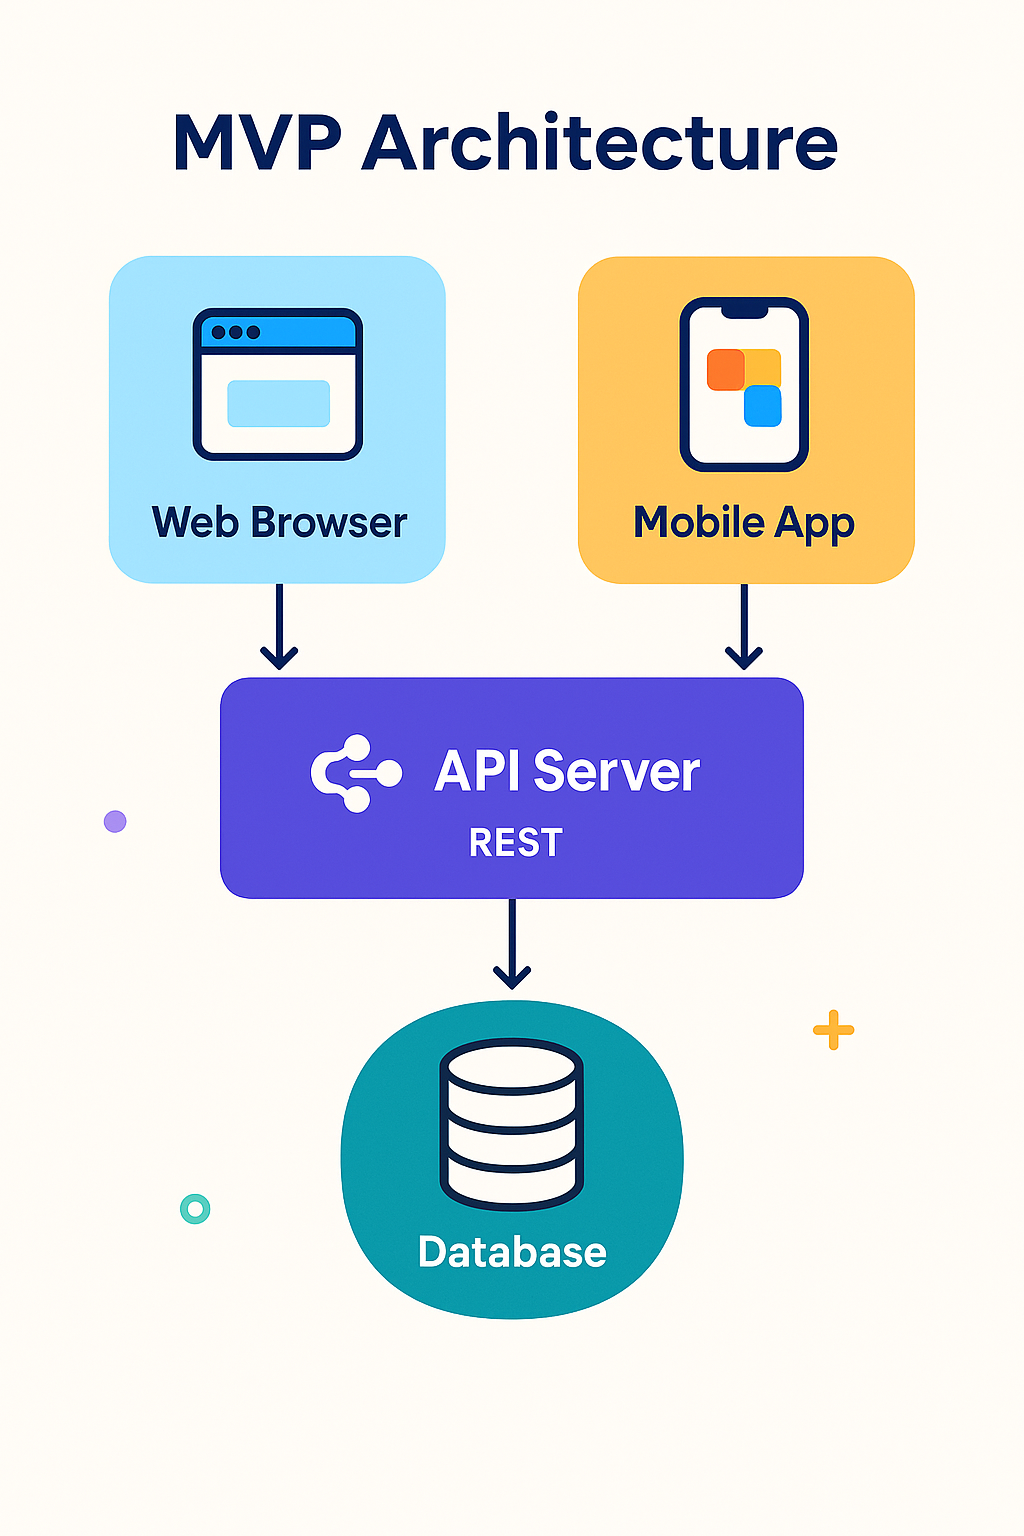
\includegraphics[width=0.5\textwidth]{images/Archi_mvp.png}
	\caption{Architecture technique du MVP 1}
\end{figure}

\section{Planification / Roadmap}
\begin{enumerate}
	\item \textbf{Semaine 1 :} Mise en place du projet backend (API .NET, PostgreSQL, AuthService). 
	\item \textbf{Semaine 2 :} Implémentation du TodoService (CRUD).
	\item \textbf{Semaine 3 :} Mise en place du frontend Angular (Auth, Todos).
	\item \textbf{Semaine 4 :} Intégration frontend-backend + tests utilisateurs.
\end{enumerate}
\subsection{Plan de tests}
\begin{itemize}
	\item Tests unitaires backend (Domain, Application).
	\item Tests intégration API Auth et Todo.
	\item E2E frontend : parcours inscription → création → complétion.
\end{itemize}

\subsection{Jalons MVP1}
\begin{enumerate}
	\item \textbf{Alpha} (S2-3) : Auth + création/liste tâches.
	\item \textbf{Beta} (S4-5) : Filtres/recherche, validations, tests intégration.
	\item \textbf{Release} (S6) : Durcissement sécurité, perfs, doc finalisée.
\end{enumerate}

\section{Conclusion}
Le MVP 1 permettra de valider la faisabilité technique du projet OrganisX et de fournir une base solide pour les fonctionnalités futures. L’approche incrémentale et modulaire garantit que chaque évolution du projet se construit sur des fondations fiables.
